\documentclass{file/TA-ITS}
\makeatletter
\def\cleardoublepage{\clearpage%
	\if@twoside
	\ifodd\c@page\else
	\vspace*{\fill}
	\hfill
	\begin{center}
		\emph{ }
	\end{center}
	\vspace{\fill}
	\thispagestyle{empty}
	\newpage
	\if@twocolumn\hbox{}\newpage\fi
	\fi
	\fi
}
\makeatother
\theoremstyle{definition}
\newtheorem{defn}{Definisi}[section]
\theoremstyle{plain}
\newtheorem{teo}[defn]{Teorema}
\newtheorem{thm}{Teorema}[section]
\newtheorem{lemma}[defn]{Lemma}
\newtheorem{lemmas}[thm]{Lemma}
\newtheorem{cor}[defn]{Akibat}
\theoremstyle{definition}
\newtheorem{con}[defn]{Contoh}
\newtheorem{prop}[defn]{Proposisi}
\renewcommand{\proofname}{Bukti}
\renewcommand{\thethm}{\arabic{chapter}.\arabic{thm}}

\newcommand{\norm}[1]{\left\|#1\right\|} % Fungsi norm (||x||)

\newcommand\firstPar{0.75cm} % Indentasi 0.75cm pada tiap paragraf (manual untuk hspace)
\setlength{\parindent}{0.75cm} % Indentasi 0.75cm pada tiap paragraf

\usepackage{fancyhdr}
\pagestyle{fancy}
\renewcommand{\headrulewidth}{0pt}
\fancyhf{}
\usepackage{ifthen}
\fancyfoot[R]{\thepage}

\usepackage[labelsep=quad]{caption}
\captionsetup[table]{skip=5pt}

\usepackage{multirow}
\usepackage{longtable}

%%% Pewarnaan code
\usepackage{color}
\usepackage{listings}

\usepackage{afterpage}

\definecolor{codegreen}{rgb}{0,0.6,0}
\definecolor{codeblack}{rgb}{0,0,0}
\definecolor{codepurple}{rgb}{0.58,0,0.82}
\definecolor{backcolour}{rgb}{0.95,0.95,0.92}

\lstdefinestyle{mystyle}{
    commentstyle=\color{codegreen},
    keywordstyle=\color{magenta},
    numberstyle=\tiny\color{codeblack},
    stringstyle=\color{codepurple},
    basicstyle=\ttfamily\footnotesize,
    breakatwhitespace=false,
    breaklines=true,
    captionpos=b,
    keepspaces=true,
    numbers=left,
    numbersep=5pt,
    showspaces=false,
    showstringspaces=false,
    showtabs=false,
    tabsize=2
}
%%% Pewarnaan code

\hypersetup{ % Merubah warna link
    colorlinks,
    linkcolor={black},
    citecolor={black},
    urlcolor={black}
}

% \tolerance=1
% \emergencystretch = \maxdimen
% \hyphenpenalty=10000
% \hbadness=1000

\begin{document}
\newcommand\blankpage{%
    \null
    \thispagestyle{empty}%
    \addtocounter{page}{-1}%
    \newpage}

\newcommand{\foreign}[1]{\emph{#1}}

\newcommand{\thpr}{\foreign{theorem prover}}

\newcommand{\icmraw}{\operatorname{Cl}_{p+1,q+1}(\mathbb{R}) \cong \mathrm{M}_2(\operatorname{Cl}_{p,q}(\mathbb{R}))}

\newcommand{\icm}{$\icmraw$}

\newcommand{\edom}[1]{{\mathrm{End}\ #1}}

\Judul{Formalisasi Isomorfisma antara Aljabar Matriks dan Aljabar Clifford menggunakan Lean}

\JudulEng{Formalizing Ishomorphism Between Matrix Algebra and Clifford Algebra with Lean}

\Nama{Fikri Yudhistira Ajiwijaya}

\NamaKecil{Fikri Yudhistira Ajiwijaya}

\NRP{5002211165}

\Departemen{Matematika}

\Department{Mathematics}

\BidangStudi{RMK}

\Bulan{Februari} % Masuk lembar pengesahan

\Tahun{2025}

\TanggalDisetujui{23 Juni 2022} % Masuk lembar orisinilitas

\Fakultas{Sains dan Analitika Data}

\SingkatanFakultas{FSAD}

\Faculty{Scientics}

\SingkatanFakultasEng{SCIENTICS}

\Pembimbing
    {Dr. mont. Kistosil Fahim, S.Si, M.Si}
    {Muhammad Syifa'ul Mufid, S.Si., M.Si., D.Phil.}


\NIPPembimbing
    {199105222015041001}
    {198909112014041001}


\Penguji{Penguji 1}
        {Penguji 2}
        {Penguji 3}

\NIPPenguji{NIP Penguji 1}
           {NIP Penguji 2}
           {NIP Penguji 3}
\Kadep{Nama Kadept}

\NIPKadep{NIP Pak Kadept}

\BagianAwal
\LembarJudul
\TitlePage
\LembarPengesahan
\begin{Abstrak}

Tugas akhir ini bertujuan untuk memformalisasi isomorfisma antara aljabar matriks dan aljabar Clifford, khususnya \icm{}, menggunakan Lean \thpr{}. Aljabar Clifford menyediakan struktur yang menggeneralisasi bilangan kompleks dan kuaternion, dengan aplikasinya yang penting di berbagai bidang seperti analisis diferensial, analisis harmonik, geometri, dan fisika matematis. Konstruksi aljabar ini telah diformalisasikan dalam Lean oleh Wieser, beserta beberapa isomorfisma ke struktur matematika lainnya, namun isomorfisma spesifik yang dibahas dalam penelitian ini belum diformalisasikan. Seiring dengan semakin kompleksnya pembuktian matematika, verifikasi formal menjadi semakin penting untuk memastikan kebenaran hasil melalui validasi yang dibantu oleh komputer.

\katakunci{Aljabar Clifford, Aljabar Geometrik, Aljabar Matriks, Lean}

\end{Abstrak}

\begin{Abstract}

This thesis aims to formalize the isomorphism between matrix algebras and Clifford algebras, specifically \icm{}, within the Lean \thpr{}. Clifford algebras provide a powerful framework that generalizes complex numbers and quaternions, having significant applications in areas such as differential analysis, harmonic analysis, geometry, and mathematical physics. Their construction has already been formalized in Lean by Wieser, along with several isomorphisms to other mathematical structures, but the specific isomorphism in question has yet to be formalized. As mathematical proofs grow more complex, formal verification is becoming increasingly important for ensuring the correctness of results through computer-assisted validation.\keywords{Clifford Algebra, Geometric Algebra, Matrix Algebra, Lean}

\end{Abstract}
\DaftarIsi\raggedbottom
\DaftarGambar
\DaftarTabel
\DaftarSimbol
\begin{flushleft}
\begin{tabular}{lrl}

$\oplus$ &:& Operasi direct sum

\end{tabular}
\end{flushleft}
\BagianInti
\chapter{PENDAHULUAN}
\section{Latar Belakang}

Aljabar Clifford digunakan dalam berbagai bidang matematika: 1) bidang analisis diferensial, digunakan dalam pembuktian teorema indeks Atiyah-Singer; 2) bidang analisis harmonik, sedemikian transformasi Riesz memberikan generalisasi dimensi lebih tinggi dari transformasi Hilbert; 3) bidang geometri, menjelaskan struktur grup klasik melalui grup spin; 4) bidang fisika matematis, yang mana aljabar Clifford menyediakan kerangka untuk teori elektromagnetik, partikel spin 1/2, dan operator Dirac dalam mekanika kuantum relativistik \citep{Garling2011}. Aljabar ini menggeneralisasi bilangan kompleks dan kuaternion, secara elegan menghubungkan geometri dan aljabar. Aljabar ini dapat menyatukan empat persamaan Maxwell menjadi satu ekspresi. Dan aljabar ini memiliki penggunaan yang menarik di bidang komputer grafis, komputasi visual, dan robotika \citep{Wieser2024}. Dengan aplikasinya yang luas ini, banyaklah alasan kuat untuk mempelajari aljabar Clifford, karena aljabar ini menawarkan alat yang efektif untuk eksplorasi teoretis maupun pemecahan masalah praktis.

Di era di mana bukti matematika telah menjadi begitu panjang hingga menyerupai novel, kemungkinan terjadinya kesalahan manusia semakin meningkat. Hal ini menimbulkan kebutuhan untuk verifikasi formal yang memungkinkan komputer untuk membantu memeriksa kebenaran bukti \citep{Palmer2020}. Sebagai contoh adalah konjektur Kepler, dibuktikan pada tahun 1993, tetapi karena bukti tersebut sangat rumit sehingga masih ada keraguan mengenai kebenarannya. Akhirnya konjektur tersebut berhasil selesai diformalisasikan di tahun 2014 \citep{Tao2024}. Sebagai contoh lain, bukti awal Andrew Wiles untuk Fermat's Last Theorem mengandung kesalahan yang harus dikoreksi, mengilustrasikan bagaimana penggunaan alat verifikasi bisa membantu Wiles mengidentifikasi kesalahan itu lebih awal \citep{Palmer2020}. Hal-hal ini menunjukkan bahwa verifikasi formal akan menjadi bagian penting dari masa depan matematika.

Lean adalah \thpr{} yang dikembangkan di Microsoft Research dan Carnegie Mellon University. Lean memiliki kernel kecil yang terpercaya, yang didasarkan pada dependent type theory. Saat ini, Lean digunakan untuk memformalkan teori kategori, teori tipe homotopi, dan aljabar abstrak \citep{Moura2015}. Konstruksi aljabar Clifford telah diformaliksikan dalam Lean oleh Wieser, dan telah ia telah menformalisasikan pula beberapa isomorfisma dalam aljabar Clifford seperti kepada bilangan riil, bilangan kompleks, bilangan dual, dan kuaternions \citep{Wieser2024}. Pada buku \cite{Lounesto2001}, terdapat  isomorfisma antara aljabar matriks dan aljabar Clifford,
\begin{align*}
    \icmraw
\end{align*}
Hasil ini belum memiliki formalisasinya dalam Lean. Pada tugas akhir ini, akan dilakukan  formalisasi hasil tersebut.

\section{Rumusan Masalah}

Berdasarkan latar belakang yang telah dibahas sebelumnya, didapat rumusan masalah pada topik ini adalah sebagai berikut.

\begin{enumerate} % Enumerate digunakan untuk membuat list angka
    \item Bagaimana dapat memperoleh pembuktian hasil \icm{}?
    \item Bagaimana dengan menggunakan Lean dapat memperoleh formalisasi hasil \icm{}?
\end{enumerate}

\section{Batasan Masalah}

\begin{enumerate}
    \item Tugas akhir ini hanya membahas isomorfisma antara aljabar matriks dan aljabar Clifford, tidak membahas isomorfisma lainnya.
    \item Tugas akhir ini hanya membahas isomorfisma bardasarkan hasil \icm{}, tidak untuk dari hasil lainnya.
    \item Tugas akhir ini menggunakan Lean 4, tidak Lean versi lainnya.
\end{enumerate}

\section{Tujuan}

\begin{enumerate}
    \item Mendapatkan bukti dari hasil \icm{}.
    \item Mendapatkan formalisasi dari hasil \icm{}.
\end{enumerate}

\section{Manfaat}

\begin{enumerate}
    \item Memberikan kontribusi pada upaya formalisasi matematika.
    \item Meningkatkan pemahaman tentang aljabar Clifford dan menunjukkan potensi verifikasi formal dalam matematika modern.
    \item Menghubungkan hasil teoritis abstrak dengan hasil yang dapat diverifikasi secara formal.
\end{enumerate}

\pagebreak
\chapter{TINJAUAN PUSTAKA}
\section{Penelitian Terdahulu}

Pada tahun 1960-an, Porteous menulis buku berjudul Topological Geometry, yang bertujuan untuk mempromosikan pendekatan kalkulus diferensial tanpa basis untuk fungsi-fungsi variabel banyak. Menariknya, hampir secara kebetulan, buku tersebut mencakup bagian penting tentang aljabar Clifford—sebuah generalisasi dari kuaternion yang pada waktu itu masih belum banyak dikenal. Bagi pembaca yang tertarik untuk menggali lebih dalam tentang aljabar Clifford, \citeauthor{Porteous1995} kemudian menerbitkan Clifford Algebras and the Classical Groups pada tahun \citeyear{Porteous1995}, yang memberikan penjelasan lebih mendalam mengenai topik ini.

Dalam buku Clifford Algebras and Spinors karya \cite{Lounesto2001}, dibahas struktur dan sifat-sifat aljabar Clifford, serta bagaimana aljabar ini terhubung dengan ruang spinor. Dalam buku ini, dibahas pula berbagai macam isomorfisma aljabar Clifford dengan struktur-struktur lainnya, termasuk pada matriks. Selain itu, karya \citeauthor{Lounesto2001} juga sangat relevan ketika membahas generalisasi dimensi yang lebih tinggi dari struktur aljabar, terutama dalam bidang-bidang seperti mekanika kuantum, relativitas, dan geometri diferensial. Penjelasan rinci tentang peran Clifford algebras dalam mendefinisikan representasi spinor, serta cara pengolahan masalah topologi dan geometri.

Buku Clifford Algebras: An Introduction karya \cite{Garling2011} merupakan sumber yang sangat baik untuk menggali lebih dalam mengenai aplikasi aljabar Clifford. Buku ini secara efektif menghubungkan aljabar abstrak dengan aplikasi-aplikasi dunia nyata, khususnya dalam fisika dan geometri. Garling menggambarkan bagaimana aljabar Clifford digunakan untuk mendeskripsikan spinor dalam mekanika kuantum, rotasi dalam relativitas khusus, dan objek geometri dalam geometri diferensial. Selain itu, relevansi aljabar Clifford dalam bidang-bidang seperti robotika dan komputer grafis juga dibahas, menjadikan buku ini referensi yang berharga untuk memahami baik aspek teoretis maupun praktis dari topik ini.

Theorem Proving in Lean karya \cite{Avigad2024} memberikan pengantar yang praktis untuk menggunakan Lean proof assistant dalam memformalisasi matematika. Buku ini mencakup logika dasar serta teori matematika yang lebih maju, dengan contoh dan latihan yang jelas yang menunjukkan cara menulis, memverifikasi, dan memeriksa bukti formal menggunakan Lean. Buku ini menjadi sumber yang berguna bagi mereka yang tertarik dengan verifikasi formal dan pembuktian teorema otomatis, khususnya dalam bidang matematika, ilmu komputer, dan verifikasi perangkat lunak.

Mathematics in Lean karya \cite{Avigad2025} merupakan sumber yang baik untuk eksplorasi lebih mendalam tentang penggunaan taktik dalam Lean. Buku ini berfokus pada penggunaan taktik untuk membangun dan memanipulasi ekspresi matematika kompleks, dengan pendekatan praktis dalam memformalisasi matematika menggunakan Lean. Penekanan diberikan pada cara memandu Lean dalam membangun bukti formal melalui instruksi taktik, menjadikannya referensi yang ideal untuk berinteraksi dengan Lean secara dinamis.

Esai \cite{Palmer2020} membahas ide dasar dari set theory dan type theory, dengan fokus pada dependent type theory sebagai alternatif dari set theory klasik dalam memformalkan matematika. Dijelaskan bahwa Lean menggunakan dependent type theory, yang menggabungkan logika intuisionistik melalui korespondensi "proposisi-sebagai-tipe", memberikan keuntungan praktis, terutama dalam pemrograman, karena menggunakan spesifikasi tipe yang lebih tepat. Meskipun Lean didasarkan pada logika intuisionistik, penalaran klasik masih bisa diterapkan jika diperlukan, sehingga memberikan fleksibilitas dalam formalisasi matematika. Esai ini menunjukkan bagaimana peralihan dari set theory ke type theory dapat mengubah cara matematika diformalkan dengan pendekatan yang berbeda.

Disertasi \cite{Wieser2024}, Formalizing Clifford Algebras and Related Constructions in the Lean Theorem Prover, adalah formalisasi struktur aljabar Clifford dalam Lean. Ini menjadi landasan yang penting pada tugas akhir ini, sebab untuk melakukan formalisasi \icm{}, diperlukan adanya implementasi struktur aljabar Clifford yang dapat digunakan. Pada disertasi tersebut, telah dilakukan pula beberapa formalisasi isomorfisma aljabar Clifford pada struktur lainnya. Strategi formalisasi yang digunakan oleh Wieser dapat dijadikan inspirasi dalam upaya formalisasi di tugas akhir ini.

\section{Aljabar Clifford}

Aljabar Clifford dapat didefinisikan dengan beberapa cara, seperti oleh aljabar eksterior, oleh \foreign{universal property}, dan oleh ideal dari aljabar tensor \citep{Lounesto2001}. Pada tinjauan ini, dikonstruksikan aljabar Clifford sebagai ideal dari aljabar tensor.

\begin{defn}[Grup]
Himpunan $G$ dengan operasi $+$ yang memenuhi sifat-sifat
\begingroup
\allowdisplaybreaks
\begin{align*}
    \forall a,b,c \in G,&& a + (b + c) &= (a + b) + c \\
    \exists 0 \in G, \forall a \in G,&& a + 0 &= a \\
    \exists 0 \in G, \forall a \in G,&& 0 + a &= a \\
    \forall a \in G, \exists {-a} \in G,&& a + {-a} &= 0 \\
    \forall a \in G, \exists {-a} \in G,&& {-a} + a &= 0
\end{align*}
\endgroup
adalah grup G \citep{Jacobson1995}.
\end{defn}

\begin{defn}[Grup Abelian]
Grup $G$ yang memenuhi sifat
\begin{align*}
    \forall a,b \in G,&& a + b &= b + a
\end{align*}
adalah grup abelian $G$ \citep{Jacobson1995}.
\end{defn}

\begin{defn}[Homomorfisma Grup]
Misalnya $G$ dan $H$ adalah grup, pemetaan ${\eta: G \to H}$ yang memenuhi sifat
\begin{align*}
    \forall a,b \in G,&& \eta(a+b) &= \eta(a) + \eta(b)
\end{align*}
adalah homomorfisma grup \citep{Jacobson1995}.
\end{defn}

\begin{defn}[Endomorfisma]
Misalnya $G$ adalah grup, homomorfisma $G$ ke dirinya sendiri, ${\eta: G \to G}$, adalah endomorfisma \citep{Jacobson1995}.
\end{defn}

\begin{defn}[Ring]
Himpunan $R$ dengan dua operasi $+$ dan $\cdot$ yang memenuhi grup abelian $R$ untuk operasinya $+$ dan memenuhi sifat-sifat
\begingroup
\allowdisplaybreaks
\begin{align*}
    \forall a,b,c \in R,&& a(bc) &= (ab)c \\
    \exists 1 \in R, \forall a \in R,&& a1 &= a \\
    \exists 1 \in R, \forall a \in R,&& 1a &= a \\
    \forall a,b,c \in R,&& a(b+c) &= ab + ac \\
    \forall a,b,c \in R,&& (a+b)c &= ac + bc
\end{align*}
\endgroup
adalah ring $R$ \citep{Jacobson1995}.
\end{defn}

\begin{defn}[Ring Komutatif]
Ring $R$ yang memenuhi sifat
\begin{align*}
    \forall a,b \in R,&& ab &= ba
\end{align*}
adalah ring komutatif $R$ \citep{Jacobson1995}.
\end{defn}

\begin{defn}[Homomorfisma Ring]
Misalnya $R$ dan $S$ adalah ring, pemetaan ${\eta: R \to S}$ yang memenuhi homomorfisma grup dan memenuhi sifat-sifat
\begingroup
\allowdisplaybreaks
\begin{align*}
    \forall a,b \in R,&& \eta(ab) &= \eta(a)\eta(b) \\
    \exists 1 \in R, \forall a \in R,&& \eta(a)\eta(1) &= \eta(a) \\
    \exists 1 \in R, \forall a \in R,&& \eta(1)\eta(a) &= \eta(a)
\end{align*}
\endgroup
adalah homomorfisma ring \citep{Jacobson1995}.
\end{defn}

\begin{defn}[Anti-homomorfisma Ring]
Misalnya $R$ dan $S$ adalah ring, pemetaan ${\eta: R \to S}$ yang memenuhi homomorfisma grup dan memenuhi sifat-sifat
\begingroup
\allowdisplaybreaks
\begin{align*}
    \forall a,b \in R,&& \eta(ab) &= \eta(b)\eta(a) \\
    \exists 1 \in R, \forall a \in R,&& \eta(a)\eta(1) &= \eta(a) \\
    \exists 1 \in R, \forall a \in R,&& \eta(1)\eta(a) &= \eta(a)
\end{align*}
\endgroup
adalah anti-homomorfisma \citep{Jacobson1995}.
\end{defn}

\begin{defn}[Ring dari Himpunan Endomorfisma Grup Abelian]
Misalnya $M$ adalah grup abelian, $\edom{M}$ adalah himpunan endomorfima $M$. Didefinisikan operasi ${\eta + \zeta}$,
\begin{align*}
	\forall \eta,\zeta \in \edom{M}, \forall x \in M,&& (\eta + \zeta)(x) &= \eta(x) + \zeta(x)
\end{align*}
yang merupakan endomorfisma $M$, maka ${\eta + \zeta \in \edom{M}}$. Kemudian, diketahui operasi komposisi $\eta\zeta$
\begin{align*}
	\forall \eta,\zeta \in \edom{M}, \forall x \in M,&& (\eta\zeta)(x) &= \eta(\zeta(x))
\end{align*}
yang jelas $\eta\zeta \in \edom{M}$. Didapatkan $\edom{M}$ memenuhi
\begingroup
\allowdisplaybreaks
\begin{align*}
    \forall \eta,\zeta,\rho \in \edom{M}, \forall x \in M,&& (\eta + (\zeta + \rho))(x) &= ((\eta + \zeta) + \rho)(x) \\
    \exists 0 \in \edom{M}, \forall \eta \in \edom{M}, \forall x \in M,&& \eta(x) + 0(x) &= \eta(x) \\
    \exists 0 \in \edom{M}, \forall \eta \in \edom{M}, \forall x \in M,&& 0(x) + \eta(x) &= \eta(x) \\
    \forall \eta \in \edom{M}, \exists {-\eta} \in \edom{M}, \forall x \in M,&& \eta(x) + {-\eta(x)} &= 0 \\
    \forall \eta \in \edom{M}, \exists {-\eta} \in \edom{M}, \forall x \in M,&& {-\eta(x)} + \eta(x) &= 0 \\
    \forall \eta,\zeta \in \edom{M}, \forall x \in M,&& \eta(x) + \zeta(x) &= \zeta(x) + \eta(x) \\
    \forall \eta,\zeta,\rho \in \edom{M}, \forall x \in M,&& (\eta(\zeta\rho))(x) &= ((\eta\zeta)\rho)(x) \\
    \exists 1 \in \edom{M}, \forall \eta \in \edom{M}, \forall x \in M,&& (\eta1)(x) &= \eta(x) \\
    \exists 1 \in \edom{M}, \forall \eta \in \edom{M}, \forall x \in M,&& (1\eta)(x) &= \eta(x) \\
    \forall \eta,\zeta,\rho \in \edom{M}, \forall x \in M,&& (\eta(\zeta+\rho))(x) &= (\eta\zeta)(x) + (\eta\rho)(x) \\
    \forall \eta,\zeta,\rho \in \edom{M}, \forall x \in M,&& ((\eta+\zeta)\rho)(x) &= (\eta\rho)(x) + (\zeta\rho)(x)
\end{align*}
\endgroup
sehingga $\edom{M}$ dengan operasinya ${\eta + \zeta}$ dan $\eta\zeta$ adalah ring \citep{Jacobson1995}.
\end{defn}

\begin{defn}[Modul Kiri]
Misalkan $R$ adalah ring dan $M$ adalah grup abelian. Modul kiri atas $R$, disebut juga modul-$R$ kiri, adalah grup abelian $M$ bersama dengan pemetaan ${(a, x) \to ax : R \times M \to M}$ yang memenuhi sifat-sifat
\begingroup
\allowdisplaybreaks
\begin{align*}
    \forall a \in R, \forall x,y \in M,&& a(x + y) &= ax + ay \\
    \forall a,b \in R, \forall x \in M,&& (a + b)x &= ax + bx \\
    \forall a,b \in R, \forall x \in M,&& (ab)x &= a(bx) \\
    1 \in R, \forall x \in M,&& 1x &= x
\end{align*}
\endgroup
Diberikan homomorfisma ring ${\eta: R \to \edom{M}}$ dan didefinisikan ${ax = \eta(a)x}$, pemetaan $ax$ memehuni sifat-sifat tersebut karena
\begingroup
\allowdisplaybreaks
\begin{align*}
    \forall a \in R, \forall x,y \in M,&& \eta(a)(x + y) &= \eta(a)(x) + \eta(a)(y) \\
    \forall a,b \in R, \forall x \in M,&& \eta(a + b)(x) &= \eta(a)(x) + \eta(b)(x) \\
    \forall a,b \in R, \forall x \in M,&& \eta(ab)(x) &= \eta(a)(\eta(b)(x)) \\
    1 \in R, \forall x \in M,&& \eta(1)x &= x
\end{align*}
\endgroup
Perhatikan bahwa pemetaan ${(a, x) \to ax : (R \times M) \to M}$ dapat diubah bentuk menggunakan \foreign{currying} menjadi ${\eta : R \to (M \to M)}$ \citep{Avigad2024,Jacobson1995}.
\end{defn}

\begin{defn}[Modul Kanan]
Misalkan $R$ adalah ring dan $M$ adalah grup abelian. Modul kanan atas $R$, disebut juga modul-$R$ kanan, adalah grup abelian $M$ bersama dengan pemetaan ${(x, a) \to xa : M \times R \to M}$ yang memenuhi sifat-sifat
\begingroup
\allowdisplaybreaks
\begin{align}
    \forall a \in R, \forall x,y \in M,&& (x + y)a &= xa + ya \label{eq:rm1} \\
    \forall a,b \in R, \forall x \in M,&& x(a + b) &= xa + xb \label{eq:rm2} \\
    \forall a,b \in R, \forall x \in M,&& x(ab) &= (xa)b \label{eq:rm3}  \\
    1 \in R, \forall x \in M,&& x1 &= x \label{eq:rm4}
\end{align}
\endgroup
Diberikan anti-homomorfisma ring ${\eta: R \to \edom{M}}$ dan didefinisikan ${xa = \eta(a)x}$, pemetaan $xa$ memenuhi sifat \ref{eq:rm2} karena
\begin{align*}
    \forall a,b \in R, \forall x \in M,&& \eta(ab)(x) &= \eta(b)(\eta(a)(x))
\end{align*}
dan jelas memenuhi sifat-sifat \ref{eq:rm1}, \ref{eq:rm3}, dan \ref{eq:rm4} \citep{Jacobson1995}.
\end{defn}

\begin{defn}[Modul]
Ketika $R$ adalah ring komutatif, tidak dibedakan antara modul kiri dan modul kanannya, dan disebut sebagai modul-$R$ \citep{Jacobson1995}.
\end{defn}

\begin{samepage}
\begin{defn}[Direct Sum Modul]
Misalnya $M_1$, $M_2$, ..., $M_n$ adalah modul atas ring $R$ yang sama, didefinisikan $M$ sebagai ${M_1 \times M_2 \times ... \times M_n}$, dan didefinisikan operasi
\begin{align*}
	\begin{split}
		\forall x_1,y_1 \in M_1, \forall x_2,y_2 \in M_2, ..., \forall x_n,y_n \in M_n,&&
		(x_1,x_2,...,x_n) + (y_1,y_2,...,y_n) &= (x_1+y_1,x_2+y_2,...,x_n+y_n)
	\end{split} \\
	\begin{split}
		\forall a \in $, \forall x_1 \in M_1, \forall x_2 \in M_2, ..., \forall x_n \in M_n,&&
		a(x_1,x_2,...,x_n) &= (ax_1,ax_2,...,ax_n)
	\end{split}
\end{align*}
Maka, $M$ adalah modul-$R$, dan dinotasikan sebagai ${M_1 \oplus M_2 \oplus ... \oplus M_n}$ atau ${\oplus_1^n M_i}$ \citep{Jacobson1995}.
\end{defn}
\end{samepage}

\begin{samepage}
\begin{defn}[Homomorfisma Modul]
Misalnya $R$ adalah ring komutatif, $M$ adalah modul-$R$, dan $M'$ adalah modul-$R$. Pemetaan ${\eta: M \to M'}$ yang memenuhi sifat-sifat
\begin{align*}
	\forall x,y \in M,&& \eta(x + y) = \eta(x) + \eta(y) \\
	\forall a \in R, \forall x \in M,&& \eta(ax) = a\eta(x)
\end{align*}
adalah homomorfisma modul-$R$, atau pemetaan linier-$R$.
\end{defn}
\end{samepage}

\begin{defn}[Pemetaan Biliner]
Misalnya $V$, $W$, dan $X$ adalah modul-$R$, pemetaan ${B: V \times W \to X}$ yang memenuhi sifat-sifat
\begin{align*}
	\forall v,v' \in V, \forall w \in W,&& B(v + v', w) &= B(v, w) + B(v', w) \\
	\forall v \in V, \forall w,w' \in W,&& B(v, w + w') &= B(v, w) + B(v, w') \\
	\forall \lambda \in R, \forall v \in V, \forall w \in W,&& B(\lambda v, w) &= \lambda B(v, w) \\
	\forall \lambda \in R, \forall v \in V, \forall w \in W,&& B(v, \lambda w) &= \lambda B(v, w)
\end{align*}
adalah pemetaan bilinier.
\end{defn}

\begin{samepage}
\begin{defn}[Aljabar Asosiatif]
Misalkan $R$ adalah ring komutatif dan $A$ adalah ring. $A$ bersama dengan pemetaan ${(\lambda, x) \to \lambda x : R \times A \to A}$ yang memenuhi sifat modul-$R$ dan memenuhi sifat-sifat
\begin{align*}
	\forall \lambda \in R, \forall x,y \in A,&& (\lambda x)y &= \lambda(xy) \label{eq:aa1} \\
	\forall \lambda \in R, \forall x,y \in A,&& x(\lambda y) &= \lambda(xy) \label{eq:aa2}
\end{align*}
adalah aljabar asosiatif atas $R$, disebut juga aljabar asosiatif-$R$, atau bisa lebih sederhananya aljabar-$R$.
\end{defn}
\end{samepage}

% Perhatikan bahwa misalnya $V$ adalah modul-$R$, maka $V$ adalah grup abelian, dan dengan pemetaan bilinier ${(x, y) \to xy : V \times V \to V}$, secara bersamaan $V$ dapat menjadi ring dan sekaligus memenuhi sifat-sifat \ref{eq:aa1} dan \ref{eq:aa2}, sehingga $V$ adalah aljabar asosiatif-$R$.

\begin{defn}[Homomorfisma Aljabar Asosiatif]
Misalkan $R$ adalah ring komutatif, $A$ adalah aljabar asosiatif-$R$, dan $A'$ adalah aljabar asosiatif-$R$, pemetaan ${\phi : A \to A'}$ yang memenuhi sifat-sifat
\begin{align*}
	\forall x,y \in A,&& \phi(x + y) &= \phi(x) + \phi(y) \\
	\forall x,y \in A,&& \phi(xy) &= \phi(x)\phi(y) \\
	\exists 1 \in A, \forall x \in A,&& \phi(x)\phi(1) &= \phi(x) \\
	\exists 1 \in A, \forall x \in A,&& \phi(1)\phi(x) &= \phi(x) \\
	\forall \lambda \in R, \forall x \in A,&& \phi(\lambda x) &= \lambda\phi(x)
\end{align*}
adalah homomorfisma aljabar asosiatif.
\end{defn}

\begin{defn}[Isomorfisma Aljabar Asosiatif]
Homomorfisma aljabar asosiatif yang bijektif adalah isomorfisma aljabar asosiatif.
\end{defn}

\begin{defn}[Bentuk Bilinier]
Misalnya $R$ adalah ring komutatif dan $V$ adalah modul-$R$, pemetaan ${B: V \times V \to R}$ yang memenuhi sifat-sifat
\begingroup
\allowdisplaybreaks
\begin{align*}
	\forall x,x',y \in V,&& B(x + x', y) &= B(x, y) + B(x', y) \\
	\forall x,y,y' \in V,&& B(x, y + y') &= B(x, y) + B(x, y') \\
	\forall a \in R, \forall x,y \in V,&& B(ax, y) &= aB(x, y) \\
	\forall a \in R, \forall x,y \in V,&& B(x, ay) &= aB(x, y)
\end{align*}
\endgroup
adalah bentuk bilinier $B$ pada $V$. Menggunakan induksi, $B$ dapat digeneralisasikan
\begin{align*}
	\forall a_i,b_i \in R, \forall x_i,y_i \in V,&& B(\sum_1^n a_i x_i, \sum_1^m b_j y_j) &= \sum_1^n \sum_1^m a_i b_j B(x_i, y_j)
\end{align*}
\citep{Jacobson1995}.
\end{defn}

\begingroup
\allowdisplaybreaks
\begin{defn}[Bentuk Kuadratik]
Misalnya $R$ adalah ring komutatif dan $V$ adalah modul-$R$, pemetaan ${Q: V \to R}$ yang memenuhi sifat-sifat
\begin{align*}
	\forall a \in R, \forall x \in V,&& Q(ax) &= a^2Q(x) \\
	\forall x,y \in V,&& B(x, y) &= Q(x + y) - Q(x) - Q(y)
\end{align*}
dengan $B$ bentuk bilinier, adalah bentuk kuadratik Q. Dapat dilihat jelas bahwa
\begin{align*}
	\begin{split}
		\forall a,b \in R, \forall x,y \in V,&&
		Q(ax + by) &= Q(ax) + Q(by) + B(ax,by) \\
		&= a^2 Q(x) + b^2 Q(y) + abB(x,y)
	\end{split}
\end{align*}
dan menggunakan induksi, $Q$ dapat digeneralisasikan
\begin{align*}
	Q(\sum a_i e_i) = \sum_i a_i^2 Q(e_i) + \sum_{i < j} a_i a_j B(e_i,e_j)
\end{align*}
\citep{Jacobson1995}.
\end{defn}
\endgroup

\begin{defn}[Tensor Product]
Misalnya $M$ dan $N$ adalah modul $R$. Tensor product dari $M$ dan $N$ adalah modul ${M \otimes N}$ bersama dengan pemetaan bilinier ${(u,v) \to u \otimes v : M \times N \to M \otimes N}$ yang memenuhi
\begin{enumerate}
	\item ${M \otimes N}$ digenerate sebagai modul-$R$ oleh ${\{u \otimes v : u \in M, v \in N\}}$
	\item Misalnya ${\Phi: M \times N \to P}$ adalah pemetaan bilinier modul-$R$ dimana ${\Phi(u,\star): N \to P}$ dan ${\Phi(\star,v): M \to P}$ adalah homomorfisma modul, maka terdapat homomorfisma ${\phi: M \otimes N \to P}$ sehingga ${\phi(u \otimes v) = \Phi(u, v)}$ untuk semua ${u \in M}$ dan ${v \in N}$.
\end{enumerate}
\citep{Pierce1982}.
\end{defn}

\begin{defn}[Aljabar Clifford]
Misalnya $R$ adalah ring komutatif, $V$ adalah modul-$R$, ${B: V \times V \to R}$ adalah bentuk bilinier, ${Q: V \to R}$ adalah bentuk kuadratik, $\mathcal{T}$ adalah aljabar-$R$ dari modul-$R$ dan perkalian bilinier, \foreign{quotient} dari aljabar tensor $\mathcal{T}$ oleh relasi \foreign{closure} ${v^2 = Q(v)}$ adalah aljabar Clifford \citep{Wieser2024}.
\end{defn}

\section{Dependent Type Theory}

"Teori tipe" mendapatkan namanya dari fakta bahwa setiap ekspresi memiliki tipe. Misalnya, dalam konteks tertentu, x + 0 bisa menunjukkan angka natural, sementara f bisa merujuk pada sebuah fungsi pada angka natural. Apa yang membuat teori tipe sederhana menjadi penting adalah kemampuan untuk membangun tipe-tipe baru dari tipe yang sudah ada. Sebagai contoh, jika a dan b adalah tipe, a → b menunjukkan tipe fungsi dari a ke b, dan a × b menunjukkan tipe pasangan yang terdiri dari elemen a yang dipasangkan dengan elemen b, sebuah konsep yang dikenal sebagai Cartesian Product.

Karena setiap ekspresi dalam Lean memiliki tipe, ini secara alami menimbulkan pertanyaan: tipe apa yang dimiliki oleh Type itu sendiri? Type 0 dapat dianggap sebagai alam semesta dari tipe "kecil" atau "biasa". Type 1 adalah alam semesta yang lebih besar dari tipe, yang mengandung Type 0 sebagai elemen, dan Type 2 adalah alam semesta yang bahkan lebih besar, yang mengandung Type 1 sebagai elemen. Urutan ini berlanjut tanpa batas, dengan sebuah Type n untuk setiap angka natural n. Istilah Type hanyalah singkatan dari Type 0.

Salah satu cara yang membantu untuk memahami hubungan ini adalah melalui tabel \ref{table:type-universe}, di mana pergerakan sepanjang sumbu x mewakili perubahan dalam alam semesta, dan pergerakan sepanjang sumbu y mewakili perubahan dalam apa yang disebut sebagai "derajat".

\begin{table}[H]
    \label{table:type-universe}
    \caption{Semesta Tipe  \citep{Avigad2024}}
    \centering
    \begin{tabular}{|c|c|c|c|c|}
        \hline
        sort & Prop & Type & Type 1 & Type 2 \\
        \hline
        type & True & Bool & Nat → Type & Type → Type 1 \\
        \hline
        term & trivial & true & $\lambda$ n $\mapsto$ Fin n & $\lambda$ (\_ : Type) $\mapsto$ Type \\
        \hline
    \end{tabular}
\end{table}

Beberapa operasi perlu polimorfik terhadap semesta tipe. Sebagai contoh, List $\alpha$ harus masuk akal untuk tipe $\alpha$ manapun, terlepas dari semesta tipe mana $\alpha$ berada.

Dalam dependent type theory, yang membuatnya "dependent" adalah fakta bahwa tipe-tipe dapat bergantung pada parameter. Misalnya, tipe list $\alpha$ bergantung pada argumen $\alpha$, dan ketergantungan ini membedakan list N dari list bool. Contoh lainnya adalah tipe vec $\alpha$ n, yang mewakili vektor elemen bertipe $\alpha$ dengan panjang n. Tipe ini bergantung pada dua parameter: tipe $\alpha$ : Type untuk elemen-elemen dalam vektor dan panjang n : N.

Sekarang, anggap kita ingin menulis fungsi cons yang menambahkan elemen baru di awal sebuah list. Tipe apa yang seharusnya dimiliki oleh cons? Fungsi ini bersifat polimorfik: kita mengharapkan fungsi cons untuk tipe-tipe seperti N, bool, atau tipe $\alpha$ lainnya berperilaku sama. Oleh karena itu, masuk akal jika tipe tersebut menjadi argumen pertama dari cons, sehingga untuk setiap tipe $\alpha$, cons $\alpha$ menjadi fungsi penyisipan untuk list bertipe $\alpha$. Dengan kata lain, untuk setiap $\alpha$, cons $\alpha$ adalah fungsi yang menerima elemen a : $\alpha$ dan list l : list $\alpha$, dan mengembalikan list baru. Jadi, tipe fungsi tersebut adalah cons $\alpha$ a l : list $\alpha$.

Jelas bahwa cons $\alpha$ seharusnya memiliki tipe $\alpha$ → list $\alpha$ → list $\alpha$. Tapi tipe apa yang seharusnya dimiliki oleh cons? Tebakan pertama mungkin adalah Type → $\alpha$ → list $\alpha$ → list $\alpha$, namun setelah dipikirkan lebih dalam, ini tidak masuk akal. $\alpha$ dalam ekspresi ini tidak merujuk pada apa pun, padahal seharusnya itu merujuk pada argumen bertipe Type. Dengan kata lain, dengan asumsi $\alpha$ : Type adalah argumen pertama dari fungsi, dua elemen berikutnya adalah $\alpha$ dan list $\alpha$. Tipe-tipe ini bervariasi tergantung pada argumen pertama, $\alpha$.

Hal ini mengarah pada contoh tipe Pi, atau tipe fungsi dependensi. Diberikan $\alpha$ : Type dan $\beta$ : $\alpha$ → Type, kita bisa memikirkan $\beta$ sebagai keluarga tipe-tipe yang bergantung pada $\alpha$—tipe $\beta$ a untuk setiap a : $\alpha$. Dalam hal ini, tipe $\Pi$ x : $\alpha$, $\beta$ x menunjukkan tipe fungsi f dengan sifat bahwa, untuk setiap a : $\alpha$, f a adalah elemen dari $\beta$ a. Dengan kata lain, tipe nilai yang dikembalikan oleh f bergantung pada input-nya.

Perlu dicatat bahwa $\Pi$ x : $\alpha$, $\beta$ masuk akal untuk ekspresi $\beta$ : Type apa pun. Ketika nilai dari $\beta$ bergantung pada x (seperti dalam ekspresi $\beta$ x pada paragraf sebelumnya), $\Pi$ x : $\alpha$, $\beta$ menunjukkan tipe fungsi dependensi. Ketika $\beta$ tidak bergantung pada x, $\Pi$ x : $\alpha$, $\beta$ tidak berbeda dari tipe $\alpha$ → $\beta$. Dalam dependent type theory (dan di Lean), konstruksi Pi adalah hal yang mendasar, dan $\alpha$ → $\beta$ hanya merupakan notasi untuk $\Pi$ x : $\alpha$, $\beta$ ketika $\beta$ tidak bergantung pada x.

Setiap kali kita memiliki p : Prop, kita bisa menginterpretasikan p sebagai sebuah tipe, yaitu tipe dari bukti-bukti p. Kita kemudian bisa membaca t : p sebagai pernyataan bahwa t adalah sebuah bukti dari p. Setelah kita membuat identifikasi ini, aturan-aturan untuk implikasi menunjukkan bahwa kita bisa berpindah antara p maka q dan p → q. Dengan kata lain, implikasi antara proposisi p dan q berkaitan dengan memiliki sebuah fungsi yang mengambil elemen dari p dan menghasilkan elemen dari q. Akibatnya, pengenalan konektif implikasi menjadi sepenuhnya tidak perlu: kita bisa menggunakan konstruktor ruang fungsi p → q dari dependent type theory sebagai konsep implikasi.

Ini adalah pendekatan yang diikuti dalam Kalkulus Konstruksi, dan karenanya juga dalam Lean. Aturan-aturan untuk implikasi dalam sistem pembuktian untuk deduksi alami yang sesuai dengan aturan-aturan yang mengatur abstraksi dan aplikasi fungsi merupakan sebuah contoh dari isomorfisma Curry-Howard, yang terkadang dikenal sebagai paradigma proposisi-sebagai-tipe.

Ada setidaknya dua cara untuk memandang proposisi sebagai tipe. Bagi mereka yang memiliki pandangan konstruktif terhadap logika dan matematika, ini adalah representasi yang setia dari apa yang dimaksud dengan proposisi: sebuah proposisi p mewakili semacam tipe data, yaitu spesifikasi tipe data yang membentuk sebuah bukti. Sebuah bukti dari p kemudian hanyalah sebuah objek t : p yang memiliki tipe yang sesuai.

Mereka yang tidak cenderung pada ideologi ini bisa melihatnya, sebaliknya, sebagai trik kode sederhana. Untuk setiap proposisi p, dikaitkan sebuah tipe yang kosong jika p salah dan memiliki satu elemen, sebut saja \*, jika p benar. Dalam hal ini, katakanlah bahwa (tipe yang terkait dengan) p dihuni. Kebetulan, aturan-aturan untuk aplikasi dan abstraksi fungsi dapat dengan mudah membantu kita melacak elemen-elemen mana dari Prop yang dihuni. Jadi, membangun sebuah elemen t : p memberi tahu kita bahwa p memang benar. Penghuni p dapat dianggap sebagai “fakta bahwa p itu benar.” Sebuah bukti dari p → q menggunakan “fakta bahwa p itu benar” untuk mendapatkan “fakta bahwa q itu benar”.

Saran kedua cara untuk memikirkan paradigma proposisi-sebagai-tipe ini berbeda secara mendasar. Dari sudut pandang konstruktif, bukti-bukti adalah objek matematika abstrak yang dilambangkan dengan ekspresi yang sesuai dalam dependent type theory. Sebaliknya, jika kita berpikir dalam kerangka trik kode di atas, maka ekspresi itu sendiri tidak melambangkan apa-apa yang menarik. Sebaliknya, yang menarik adalah fakta bahwa kita bisa menuliskannya dan memeriksa bahwa ekspresi tersebut ber-tipe dengan baik, yang memastikan bahwa proposisi yang dimaksud benar. Dengan kata lain, ekspresi itu sendiri adalah buktinya \citep{Avigad2024}.


\pagebreak
\chapter{METODOLOGI}
Pada bab ini akan dijelaskan secara umum mengenai urutan pelaksanaan tugas akhir dengan langkah-langkah yang dilakukan.

\section{Studi Literatur}

Pada tahap ini dilakukan identifikasi permasalahan dan mengumpulkan informasi untuk memberi acuan pemecahan permasalahan. Studi literatur digunakan untuk mempelajari dan mengkaji lebih luas mengenai identitas-identitas yang akan digunakan dalam membantu menyelesaikan tugas akhir.

\subsection{Studi Lean}

Berdasarkan saran dari Prof. Kevin Buzzard, diperlukan waktu selama 11 minggu untuk studi pengoperasian Lean dengan tingkat kesulitan yang dibutuhkan untuk formalisasi \icm{}. Oleh karena itu, akan dilakukan terlebih dahulu pembelajaran formalisasi matematika menggunakan Lean di 11 minggu awal.

\subsection{Studi Aljabar Clifford}

Dilakukan studi intensif tentang aljabar Clifford bersamaan dengan studi Lean pada 11 minggu awal.

\section{Pembuktian Isomorfisma antara Aljabar Matriks dan Aljabar Clifford}

Setelah penulis memahami aljabar Clifford, dimulailah proses pembuktian \icm{}. Diberikan waktu selama 3 minggu untuk melakukan pembuktian ini.

\section{Formalisasi Isomorfisma antara Aljabar Matriks dan Aljabar Clifford}

\subsection{Formalisasi Sifat-sifat dasar Aljabar Clifford}

Sebagai langkah awal untuk uji coba awal dilakukan formalisasi sifat-sifat dasar aljabar Clifford yang telah dipelajari pada saat studi literatur.

\subsection{Formalisasi Isomorfisma untuk Dimensi Rendah}

Setelah berhasil dilakukan formalisasi sifat-sifat dasar, dimulai proses formalisasi \icm{} untuk dimensi-dimensi rendah terlebih dahulu, yaitu untuk isomorfisma yang sudah jelas seperti pada bilangan riil ${\operatorname{Cl}_{0,0} &\cong \mathbb{R}}$, bilangan kompleks ${\operatorname{Cl}_{0,1} &\cong \mathbb{C}}$, dan kuaternion ${\operatorname{Cl}_{0,2} &\cong \mathbb{H}}$.

\subsection{Formalisasi $\operatorname{Cl}_{p+1,q+1}(\mathbf{R}) = \mathrm{M}_2(\operatorname{Cl}_{p,q}(\mathbf{R}))$}

Akhirnya, formalisasi \icm{} menggunakan Lean. Diperhitungkan waktu selama 2 minggu cukup untuk mendapatkan formalisasi hasil tersebut.

\section{Penulisan Tugas Akhir}

Setelah semua tahapan penelitian selesai, disusun laporan tugas akhir mengenai penelitian yang telah dilakukan.

\section{Diagram Alir}

Adapun diagram alir proses tugas akhir ini diilustrasikan oleh Gambar 3.1.

\begin{figure}[H]
	\centering
	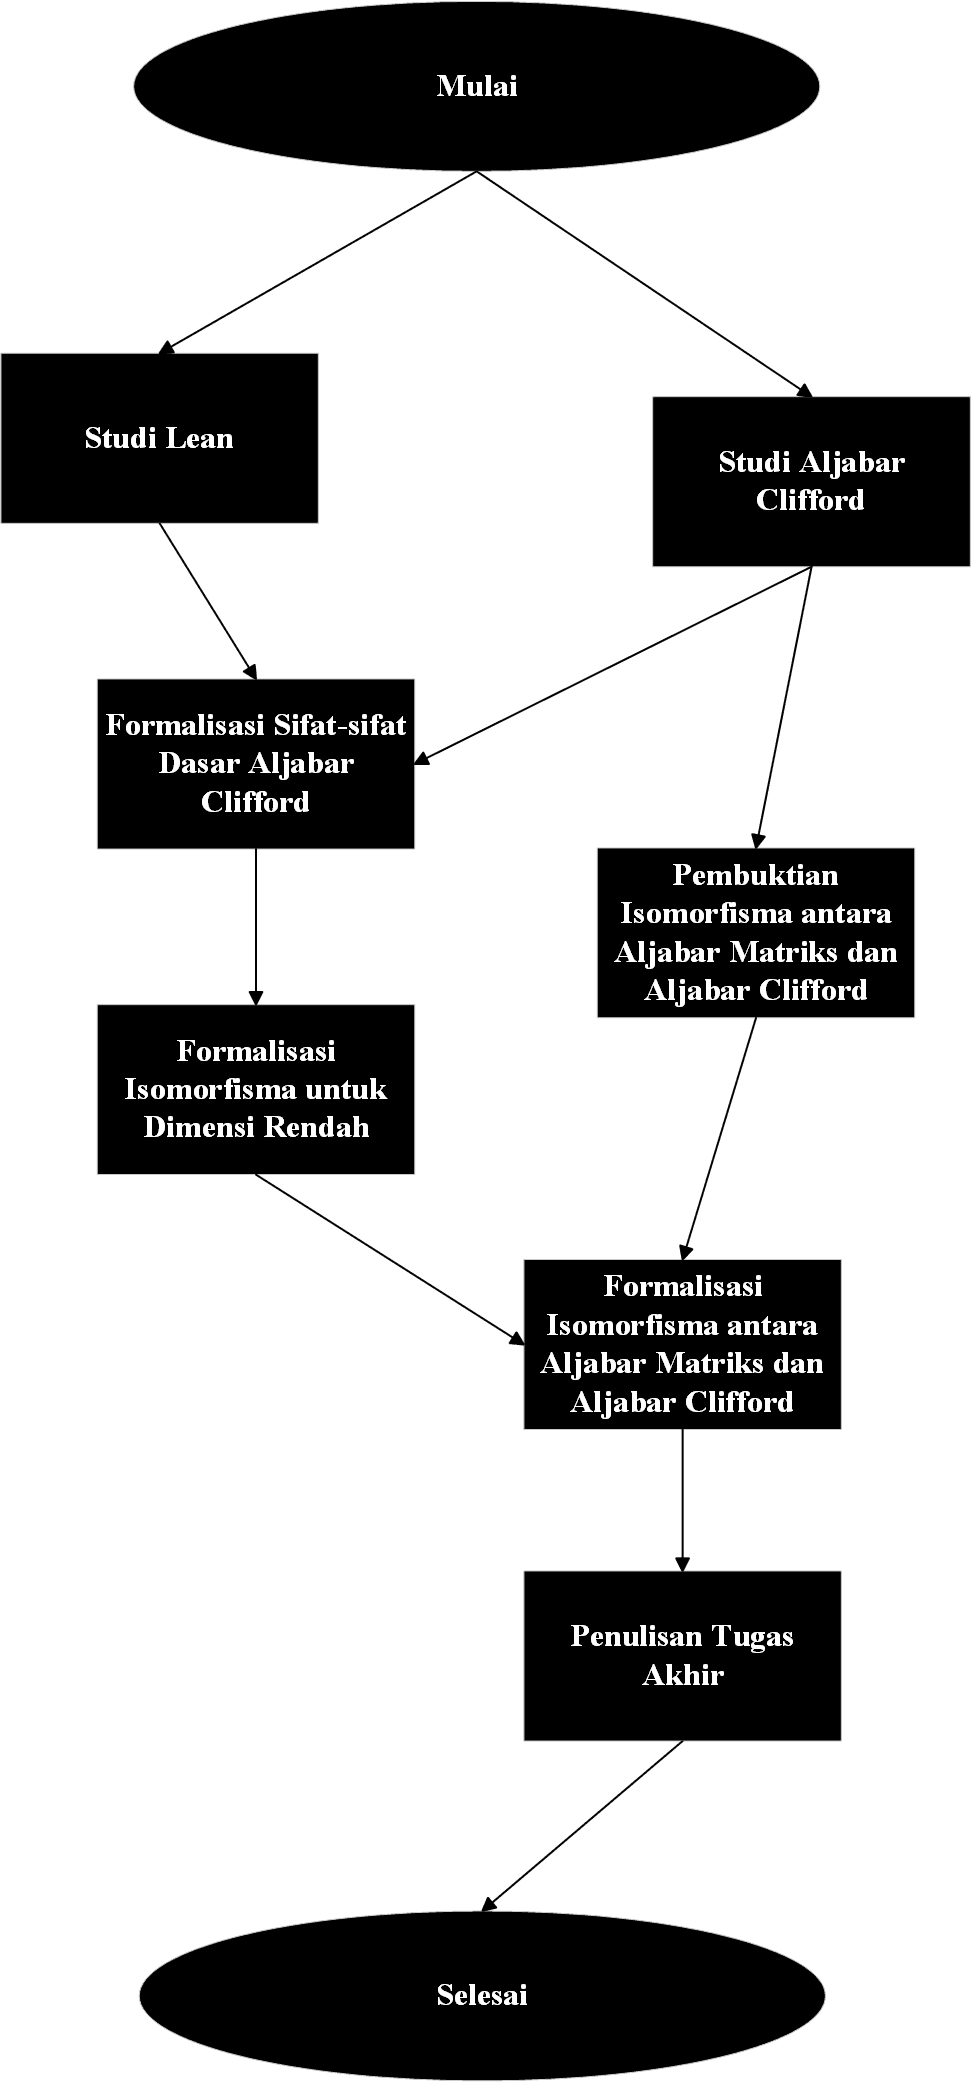
\includegraphics[width=8cm]{foto/BlockDiagram.png}
	\caption{Diagram Alir Metodologi.}
	\label{diagramalir}
\end{figure}

\section{Jadwal Kegiatan}
Berikut ini disajikan tabel jadwal kegiatan yang akan dilakukan selama 16 minggu dan berkoresponden dengan metodologi.\vspace{0.5cm}
% 	Membuat tabel

% Please add the following required packages to your document preamble:
% \usepackage{multirow}
% \usepackage[table,xcdraw]{xcolor}
% Beamer presentation requires \usepackage{colortbl} instead of \usepackage[table,xcdraw]{xcolor}
\begin{table}[H]
\caption{Jadwal Kegiatan}
\centering
\begin{tabular}{|c|l|lllllll|}
\hline
 & \multicolumn{1}{c|}{} & \multicolumn{7}{c|}{\textbf{Minggu}} \\ \cline{3-9}
\multirow{-2}{*}{\textbf{No}} & \multicolumn{1}{c|}{\multirow{-2}{*}{\textbf{Nama Kegiatan}}} & \multicolumn{1}{l|}{1 sampai 10} & \multicolumn{1}{l|}{11} & \multicolumn{1}{l|}{12} & \multicolumn{1}{l|}{13} & \multicolumn{1}{l|}{14} & \multicolumn{1}{l|}{15} & 16 \\ \hline
1 & Studi Lean & \multicolumn{1}{l|}{\cellcolor[HTML]{000000}} & \multicolumn{1}{l|}{\cellcolor[HTML]{000000}} & \multicolumn{1}{l|}{} & \multicolumn{1}{l|}{} & \multicolumn{1}{l|}{} & \multicolumn{1}{l|}{} &  \\ \hline
2 & Studi Aljabar Clifford & \multicolumn{1}{l|}{\cellcolor[HTML]{000000}{\color[HTML]{000000} }} & \multicolumn{1}{l|}{\cellcolor[HTML]{000000}} & \multicolumn{1}{l|}{} & \multicolumn{1}{l|}{} & \multicolumn{1}{l|}{} & \multicolumn{1}{l|}{} &  \\ \hline
3 & \begin{tabular}[c]{@{}l@{}}Pembuktian Isomorfisma antara\\ Aljabar Matriks dan Aljabar Clifford\end{tabular} & \multicolumn{1}{l|}{} & \multicolumn{1}{l|}{} & \multicolumn{1}{l|}{\cellcolor[HTML]{000000}{\color[HTML]{000000} }} & \multicolumn{1}{l|}{\cellcolor[HTML]{000000}{\color[HTML]{000000} }} & \multicolumn{1}{l|}{\cellcolor[HTML]{000000}{\color[HTML]{000000} }} & \multicolumn{1}{l|}{} &  \\ \hline
4 & \begin{tabular}[c]{@{}l@{}}Formalisasi Sifat-sifat Dasar\\ Aljabar Clifford\end{tabular} & \multicolumn{1}{l|}{} & \multicolumn{1}{l|}{\cellcolor[HTML]{000000}} & \multicolumn{1}{l|}{} & \multicolumn{1}{l|}{} & \multicolumn{1}{l|}{} & \multicolumn{1}{l|}{} &  \\ \hline
5 & \begin{tabular}[c]{@{}l@{}}Formalisasi Isomorfisma untuk\\ Dimensi Rendah\end{tabular} & \multicolumn{1}{l|}{} & \multicolumn{1}{l|}{} & \multicolumn{1}{l|}{\cellcolor[HTML]{000000}} & \multicolumn{1}{l|}{} & \multicolumn{1}{l|}{} & \multicolumn{1}{l|}{} &  \\ \hline
6 & \begin{tabular}[c]{@{}l@{}}Formalisasi Isomorfisma antara\\ Aljabar Matriks dan Aljabar Clifford\end{tabular} & \multicolumn{1}{l|}{} & \multicolumn{1}{l|}{} & \multicolumn{1}{l|}{} & \multicolumn{1}{l|}{\cellcolor[HTML]{000000}} & \multicolumn{1}{l|}{\cellcolor[HTML]{000000}} & \multicolumn{1}{l|}{} &  \\ \hline
7 & Penulisan Tugas Akhir & \multicolumn{1}{l|}{} & \multicolumn{1}{l|}{} & \multicolumn{1}{l|}{} & \multicolumn{1}{l|}{} & \multicolumn{1}{l|}{} & \multicolumn{1}{l|}{\cellcolor[HTML]{000000}{\color[HTML]{000000} }} & \cellcolor[HTML]{000000}{\color[HTML]{000000} } \\ \hline
\end{tabular}
\end{table}

\pagebreak
\DaftarPustaka
\end{document}
